\section{(1) Urban Prototype}\label{urban-prototype}

\begin{figure}[ht]
    \centering
    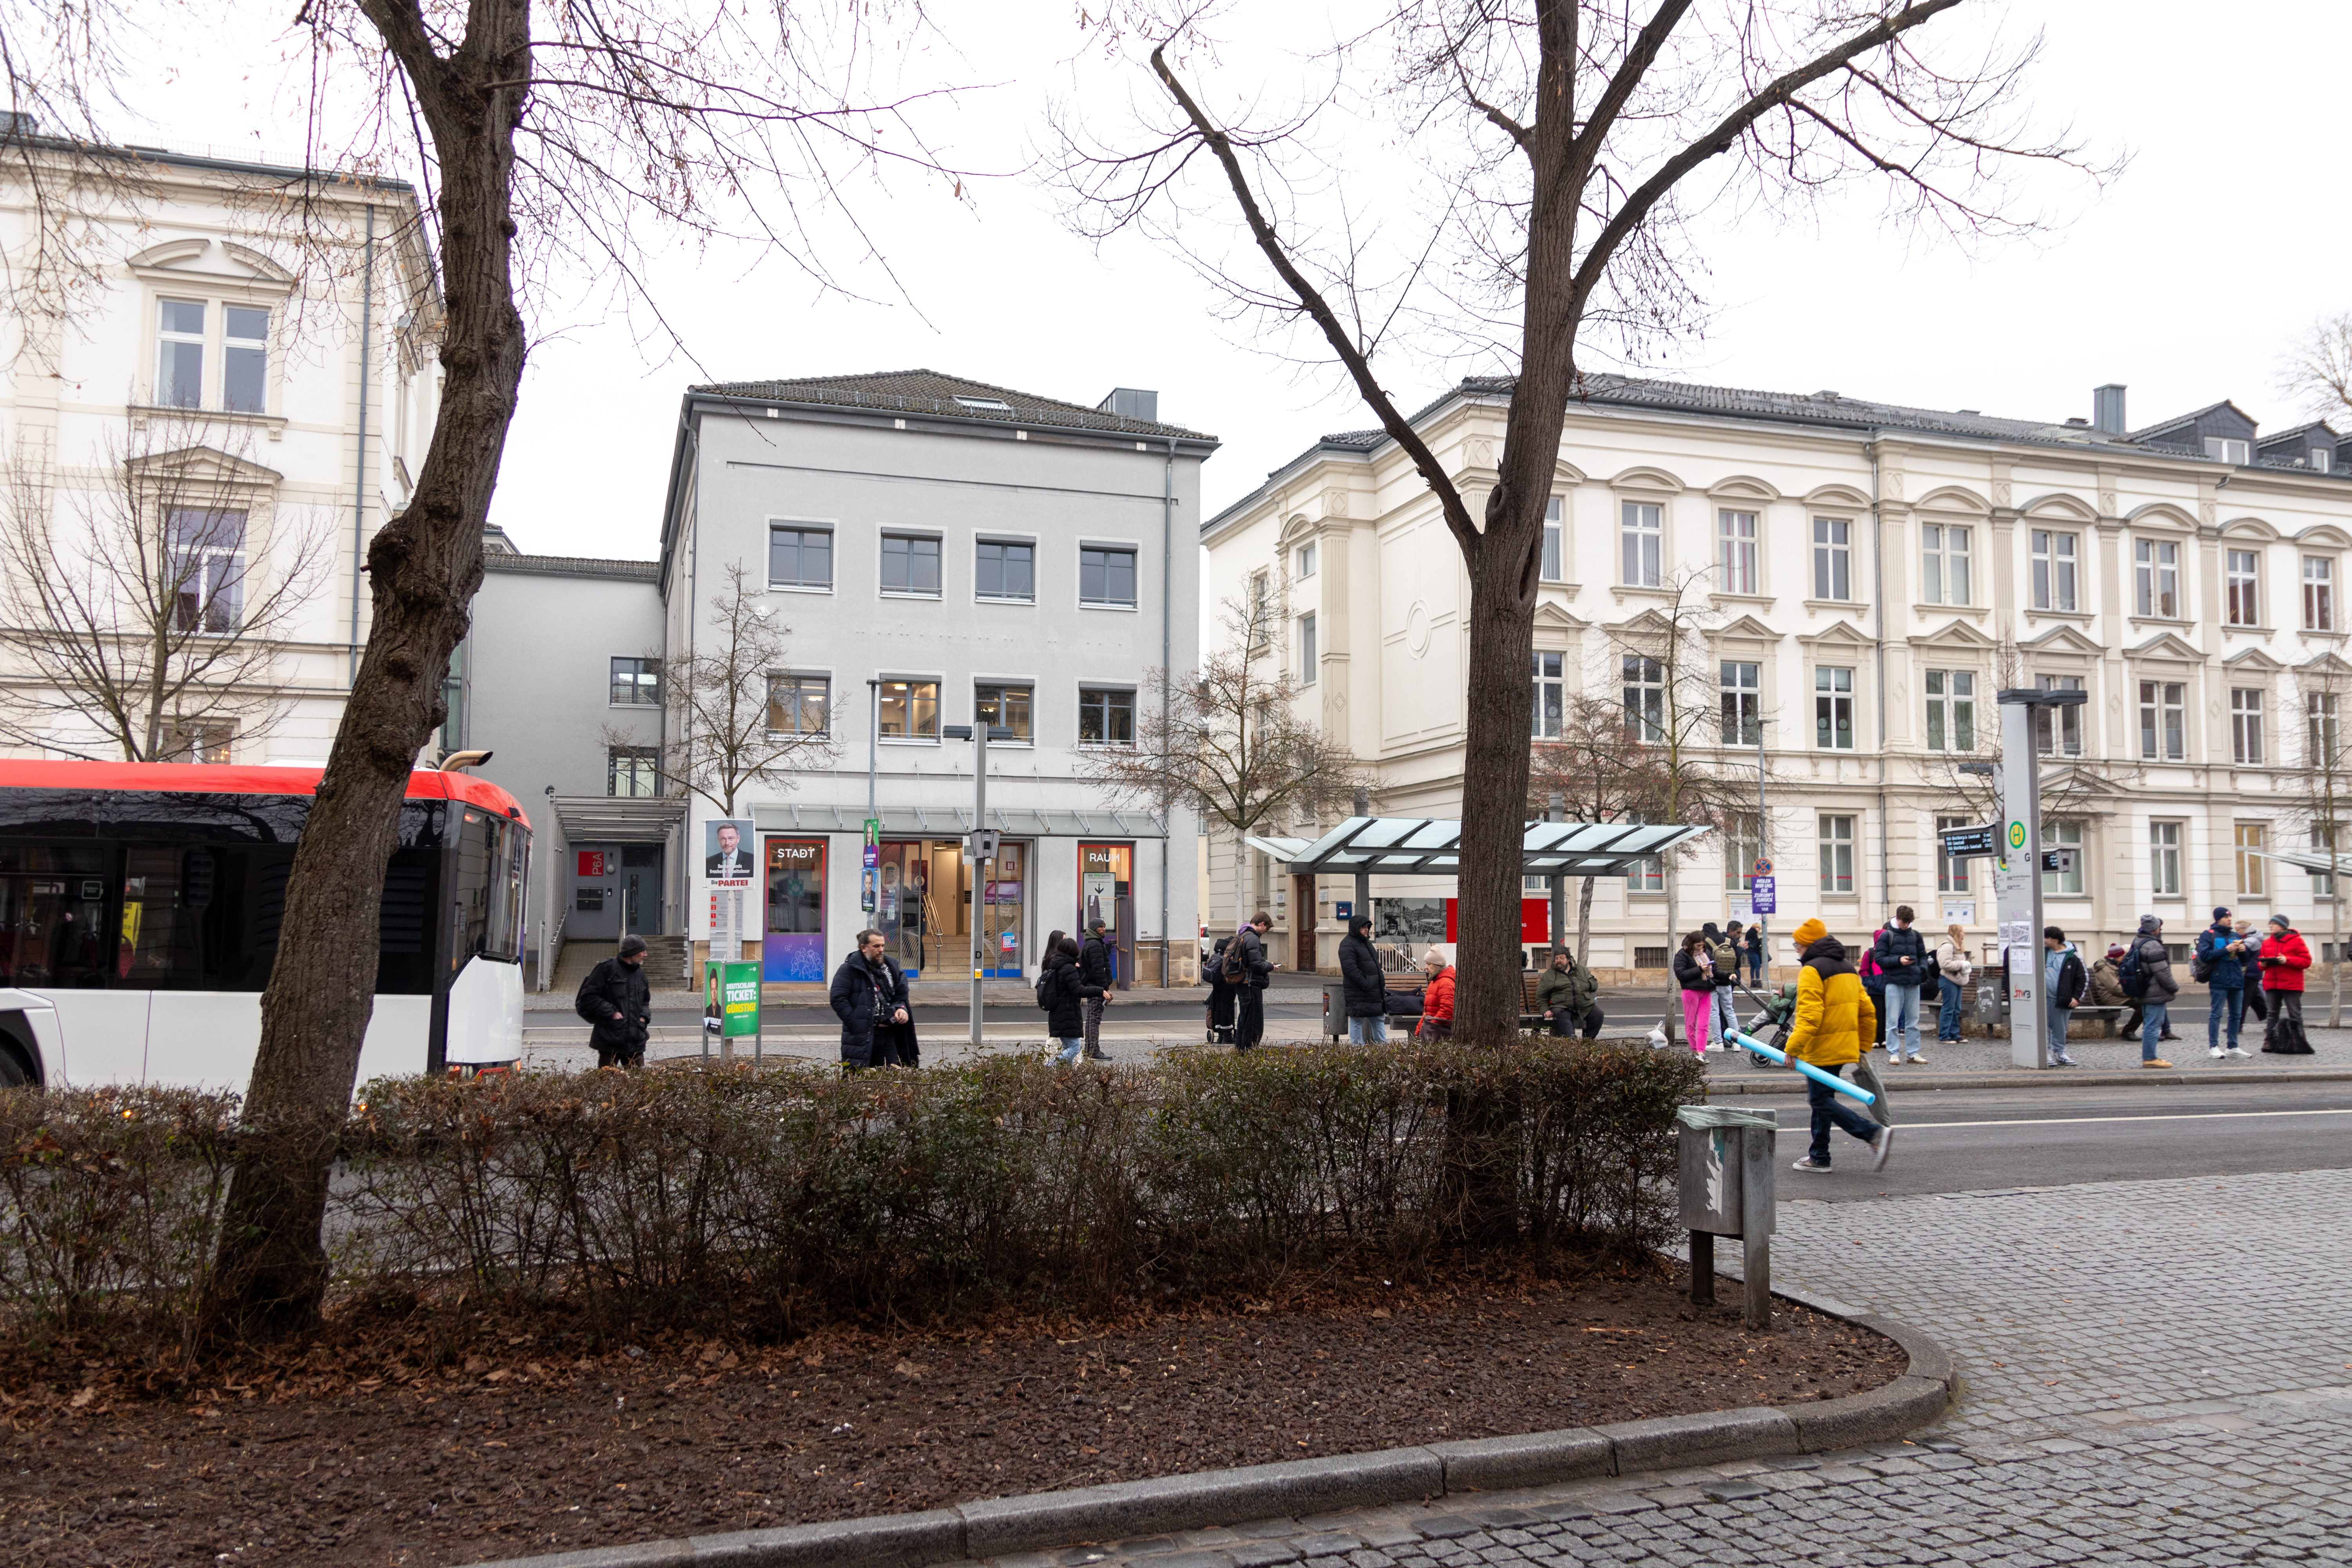
\includegraphics[width=0.8\textwidth]{figures/overview-wide.jpg}
    \caption{Situationsübersicht }
    \label{fig:urban-prototype}
\end{figure}

\subsection{Konzept}\label{konzept}

Basierend auf den in dem vorherigen Assignment identifizierten Favoriten haben wir ein finales Konzept für den Prototypen ausgearbeitet.
Dabei haben wir mit unserer ``Wahl-Quiz''-Idee begonnen, und diese iterativ zu dem im Folgenden beschriebenen Konzept einer Wahlumfrage entwickelt, die Transparenz mit dem Wahlgeheimnis verbindet.

Hierbei werden beide Public Displays am Stadt:Raum genutzt.
Vor einem der Displays wird eine Wahlkabine aufgestellt.
Interessierte Passanten können in diese Wahlkabine treten und für eine der Parteien, die bei der kommenden Bundestagswahl zur Wahl stehen, abstimmen.
Die Abstimmung erfolgt, indem die zur Partei gehörende Karte kurz in eine Wahlurne gehalten und anschließend zurückgelegt wird.
Auf dem Public Display in der Wahlkabine wird dem Teilnehmenden angezeigt, wie die Umfrage abläuft und eine Rückmeldung über die erfolgte Stimmabgabe gegeben.

Durch die Kombination aus Wahlkabine, Urne und die den Stimmzettel symbolisierenden Karten soll möglichst stark das Gefühl einer echten Wahl und dem damit verbundenen Wahlgeheimnis aufkommen.
Kontrastiert wird das einerseits durch das zweite Display, das neben den (vorläufigen) Umfrageergebnissen auch die Stimme des aktuell in der Wahlkabine stehenden Teilnehmenden dokumentiert und damit für andere Passanten sichtbar macht.
Zusätzlich sind die Wände der Wahlkabine zwar bedeckt, aber nicht wirklich blickdicht.

\subsection{Zentrale Forschungsfrage}\label{zentrale-forschungsfrage}

Unser Ziel ist es, mithilfe des Prototypen herauszufinden, wie Teilnehmer auf diesen Kontrast aus Wahlgeheimnis und Transparenz reagieren.

\subsection{Umsetzung}\label{umsetzung}

\subsubsection{Wahlkabine}\label{wahlkabine}

Die Wahlkabine ist 2 Meter hoch und hat eine Grundfläche von in etwa 80x80cm.
Der Rahmen besteht aus Holz.
Die Seiten sind mit einem dunklen Bettlagen abgehangen, um den Eindruck einer Wahlkabine zu erzeugen und den Teilnehmenden etwas Sichtschutz zu gewähren, allerdings sind die Wände damit nicht blickdicht.
Die Wahlkabine wird vor dem einen Schaufenster des Stadt:Raum positioniert und verdeckt damit die Sicht auf eines der Public Displays für Passanten, nicht aber für den aktuellen Teilnehmer in der Kabine.

\subsubsection{Urne und Stimmzettel}\label{urne-und-stimmzettel}

Die Urne ist ebenfalls aus Holz gefertigt und schwarz lackiert. Oben befindet sich ein Schlitz, in den die Wahlzettel eingesteckt werden können.
Damit die Wahlzettel beliebig wiederverwendbar sind, können diese allerdings nicht komplett, sondern nur circa 2 Zentimeter eingesteckt werden.
Die Urne ist in der Wahlkabine direkt vor dem Public Display angebracht.

Die Wahlzettel haben in etwa die Maße 8.56x7cm und sind damit so breit wie eine Standard-Kreditkarte, aber höher und etwas quadratischer.
Auf den Stimmzettel ist das Logo der entsprechenden Partei aufgedruckt.
Das Papier wurde zusammen mit einer RFID-Karte, auf der die entsprechende Partei gespeichert wurde, laminiert.

In der Urne befindet sich ein RFID-Sensor, der mit einem RaspberryPi Zero verbunden ist.
Die Stromversorgung erfolgt durch eine Powerbank.
Wenn eine Stimmkarte in die Urne gesteckt wird, erkennt der Sensor anhand der RFID-Karte die Partei und schickt einen GET-Request an den im folgenden beschriebenen Server.

\subsubsection{Public Displays}\label{public-displays}

Die beiden Public Display sind mit einem Laptop verbunden, der als Server fungiert.
Dieser empfängt die Requests vom RaspberryPi Zero in der Wahlurne und leitet die Daten an zwei Websites weiter, jeweils eine pro Public Display.
Auf dem öffentlich einsehbaren PD wird dann die aktuelle Statistik, auf dem in der Wahlkabine eine Rückmeldung über die erhaltene Stimme angezeigt.
Die Kommunikation zwischen Server und den Browsern, die die Websites anzeigen, geschieht dabei über Server-Sent Events, wodurch die Browser auch auf einem anderen Gerät laufen können.

Alle Geräte befinden sich der Einfachheit halber im selben WLAN.

\subsection{Deployment}\label{deployment}

\begin{figure}
    \centering
    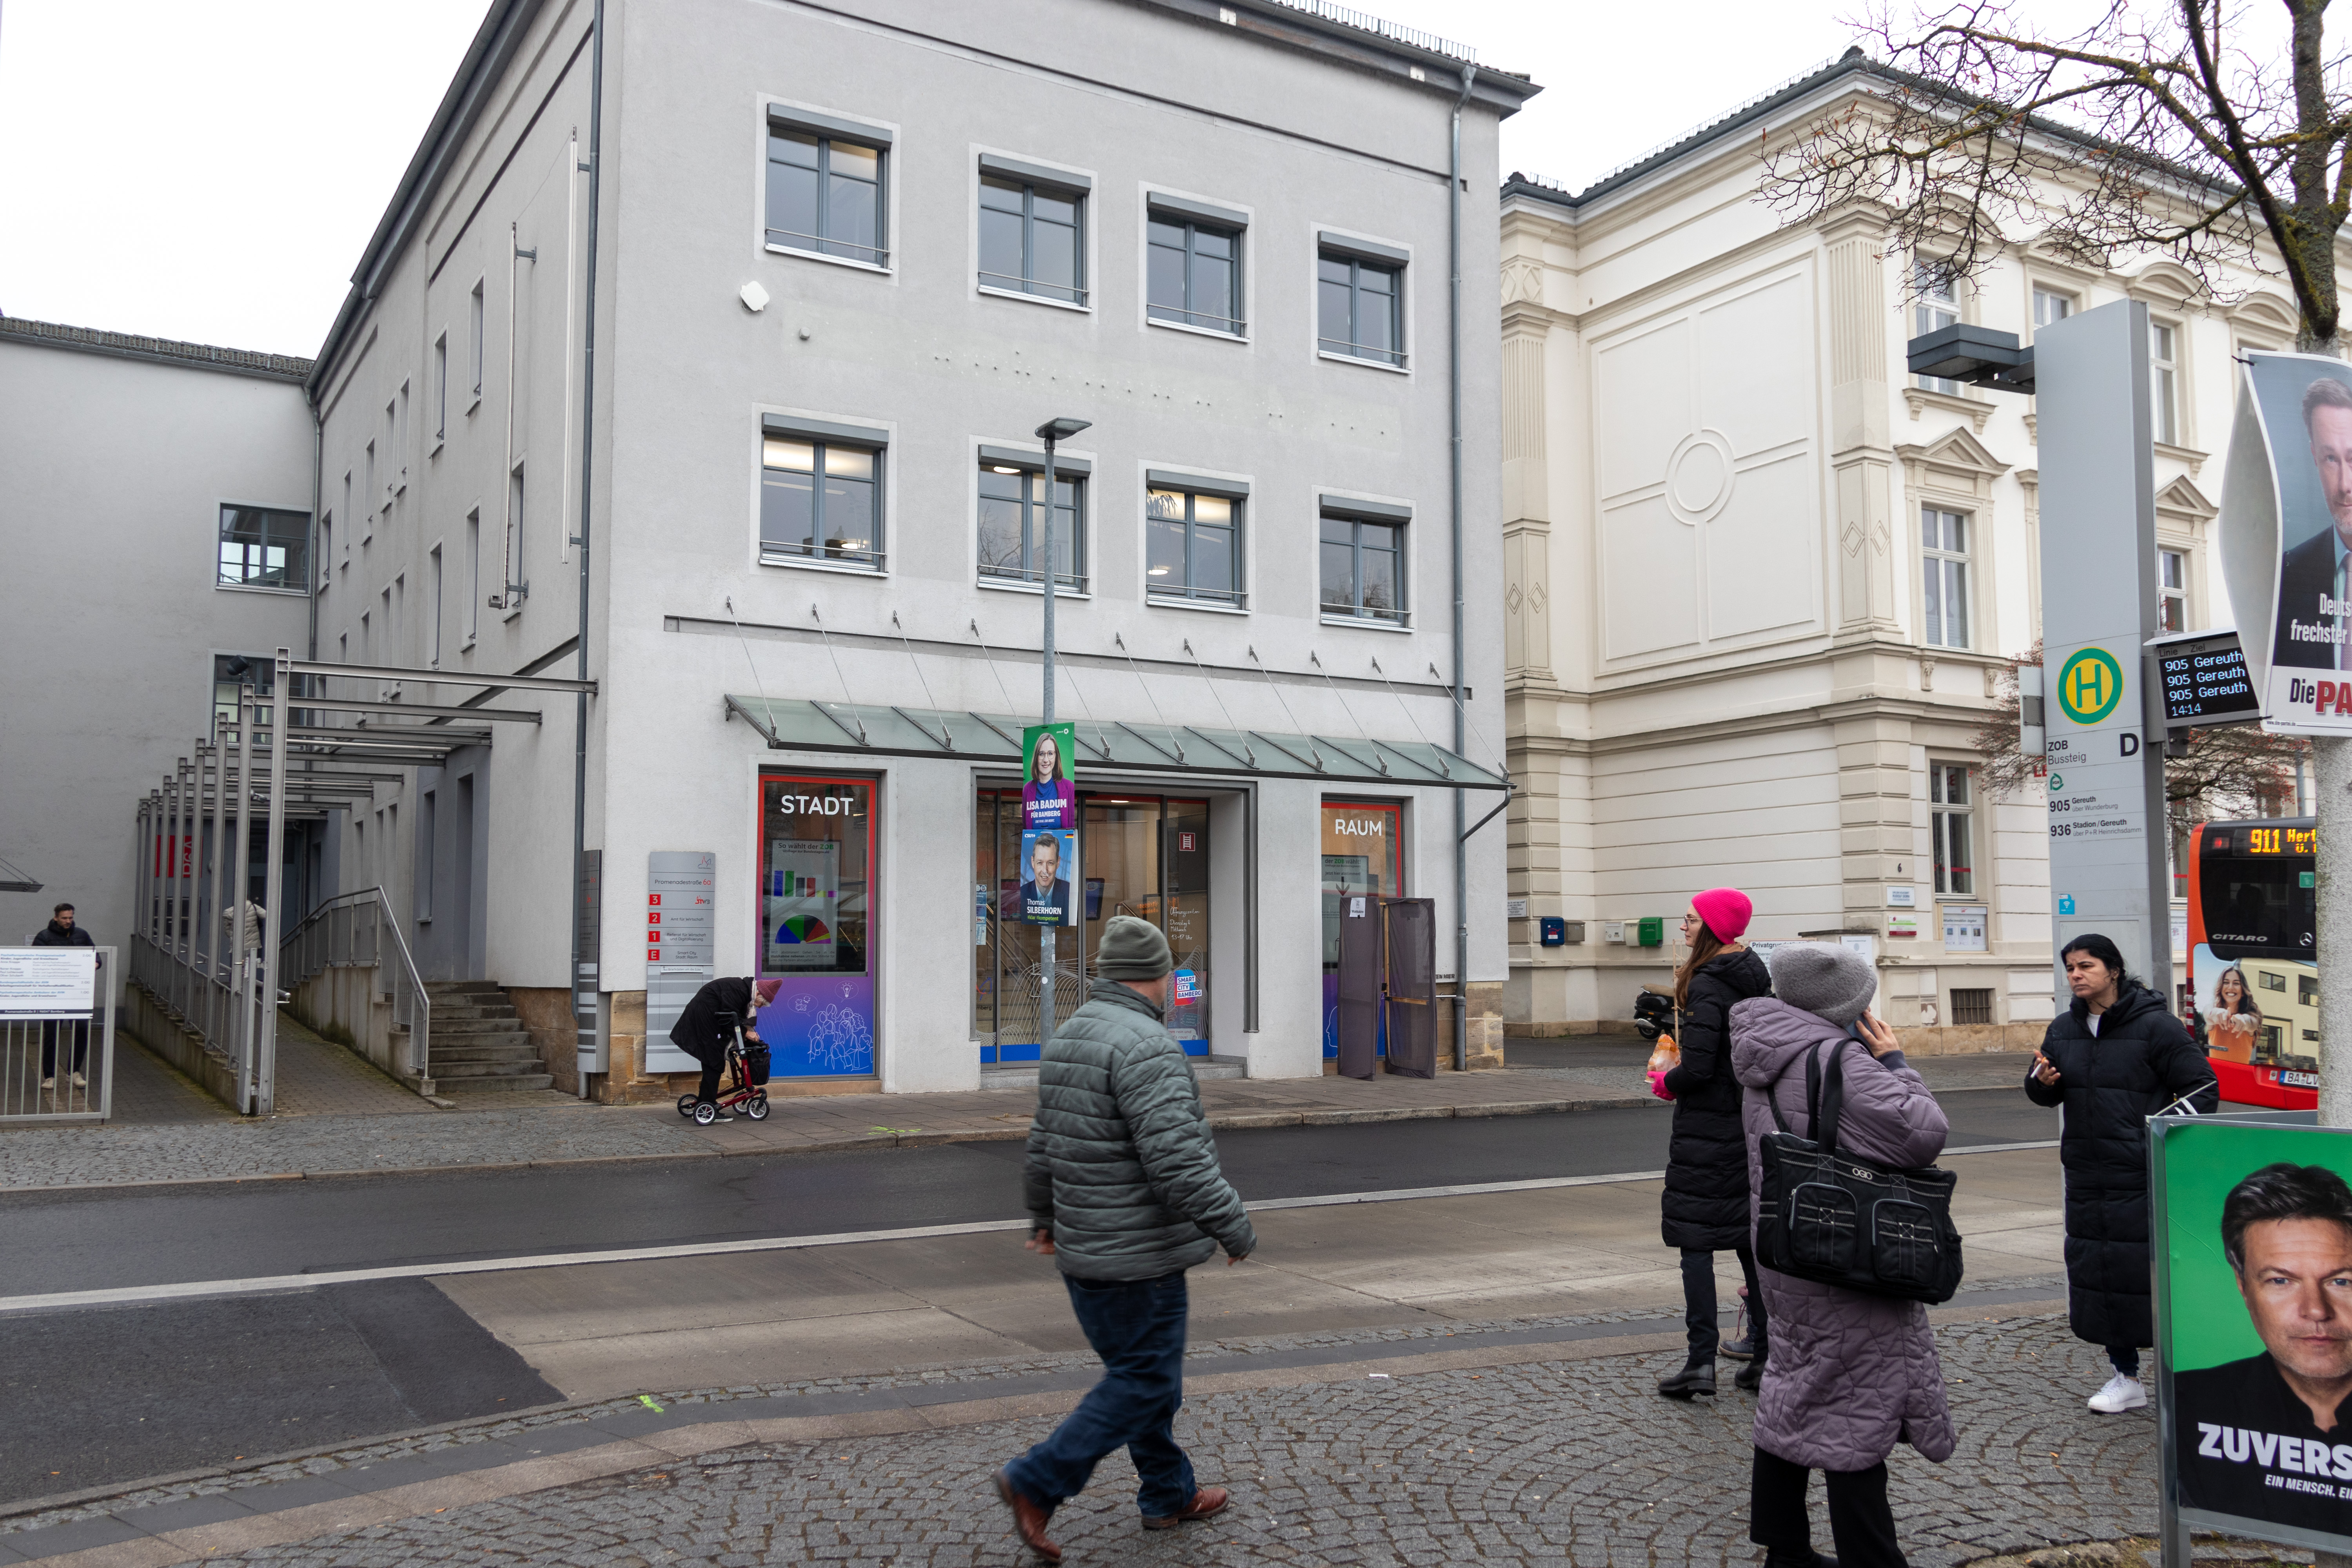
\includegraphics[width=0.8\textwidth]{figures/overview.jpg}
    \caption{Deployment des Urban Prototypen}
    \label{fig:deployment}
\end{figure}

Das Deployment wird im folgenden Kapitel ausführlich beschrieben und reflektiert.
Anbei sind zusätzlich Fotos und ein Video, das den Prototypen und Interaktionen von Passanten mit ihm zeigen.
Der verwendete Code ist auf GitHub verfügbar (\url{https://github.com/layaxx/m4_uixd-prototype}).